\phantomsection
%\addcontentsline{toc}{chapter}{Introduzione}
\chapter{Penetration Testing Report}
\markboth{Penetration Testing Report}{}

% [titolo ridotto se non ci dovesse stare] {titolo completo}
\section{Executive Summary}
Al fine di realizzare il progetto del corso \emph{Penetration Testing and Ethical Hacking} sono state svolte delle attività di Penetration Testing su una macchina virtuale vulnerabile chiamata \textbf{De-ICE S1.140}. Il fine ultimo di tutte le attività svolte è stato semplicemente didattico, con lo scopo di acquisire al meglio tutte le conoscenze fornite durante lo svolgimento del corso. Per l'esecuzione di tutte le attività è stata adottata una strategia di analisi \emph{Black-Box}, quindi senza avere nessuna conoscenza pregressa sull'asset, e sono state realizzate all'interno di un'ambiente simulato con una connessione diretta con l'asset.\\
Durante le varie attività svolte sono state riscontrate diverse vulnerabilità che possono portare un malintenzionato ad ottenere documenti o file a cui non dovrebbe avere accesso e, nel caso peggiore, alla compromissione totale del sistema.

Lasciare il sistema in questo stato è un rischio \textbf{{\color{bordeaux} critico}} e, per questa ragione, bisognerebbe correre subito ai ripari aggiornando il sistema, gli applicativi e nascondendo alcune informazioni \textbf{sensibili} per far tornare il sistema entro livelli di rischio \emph{accettabili}.

\section{Engagement Highlights}
Essendo un progetto universitario nell'ambito del corso \emph{Penetration Testing and Ethical hacking} ed essendo che l'ambiente su cui è effettuato l'intero processo è \emph{virtualizzato}, non ci sono \textbf{NDA} da rispettare e non ci sono vincoli sulle tecniche che è possibile utilizzare o sulle parti dell'asset da analizzare.

\section{Vulnerability Report}
Durante il processo sono state trovate varie vulnerabilità, alcune di queste con gravità \textbf{critica} e \textbf{alta}. Le principali sono le seguenti:
\begin{itemize}
    \item \emph{Information Leakage} (gravità \textbf{\color{bordeaux} critica}): alcune informazioni importanti sono salvate in maniera non protetta fornendo ad un attaccante la possibilità di compromettere le password degli utenti e dell'amministratore;
    \item Sistema Operativo Deprecato (gravità \textbf{\color{bordeaux} critica}): Il sistema operativo dell'asset non è più supportato e non riceverà più aggiornamenti di sicurezza. Pertanto, potrebbero presentarsi vulnerabilità che permettono ad attaccanti di ottenere pieno controllo della macchina;
    \item Versione deprecata di \textbf{ProFTPD} (gravità \textbf{\color{bordeaux} critica}): la versione attuale di \textbf{ProFTPD} consente ad un malintenzionato di leggere e scrivere qualunque file presente nel sistema senza doversi autenticare, quindi potrebbe scrivere un codice malevolo e eseguirlo da remoto;
    \item Versione deprecata di \textbf{OpenSSL} (gravità \textbf{\color{bordeaux} critica}): La versione di \textbf{OpenSSL} installata utilizza protocolli crittografici datati e vulnerabili, permettendo ad un attaccante di violare il traffico web verso il sistema. Inoltre, implementa una versione di \emph{SSL} che è affetta dalla nota vulnerabilità \textbf{HeartBleed}, con la quale un attaccante potrebbe compromettere sessioni web e ottenere chiavi e password salvate nel server;
    \item Versione vulnerabile di \textbf{phpMyAdmin} (gravità \textbf{\color{bordeaux} critica}): La versione di \textbf{phpMyAdmin} è vulnerabile ad un attacco che permette ad un malintenzionato di ottenere dati dal database senza dover autenticarsi;
    \item Utilizzo di password deboli (gravità \textbf{\color{red} alta}): Per l'accesso al sistema, sono state utilizzate password deboli che possono essere facilmente indovinate o forzate da un attaccante;
    \item Utilizzo di protocolli crittografici deboli (gravità \textbf{{\color{orange} medio}-{\color{red} alta}}): Le versioni di SSL e TLS utilizzate e supportate dal sistema sono deboli e non dovrebbero essere più supportate, visto che possono portare alla compromissione del traffico web;
    \item Server web \emph{Apache} malconfigurato (gravità \textbf{\color{orange} media}): Il server web invia informazioni sensibili che potrebbero aiutare un attaccante contro il server web stesso e, inoltre, non utilizza un meccanismo di sicurezza che impedisce ad un attaccante di fare operazioni all'insaputa del client e reindirizzarlo verso pagine web malevole;
    \item Utilizzo di una versione deprecata di \textbf{jQuery} (gravità \textbf{\color{orange} media}): Viene utilizzata una versione della libreria \textbf{jQuery} che è vulnerabile ad un attacco che permette ad un attaccante di rubare informazioni sensibili ai client che visitano una pagina con integrata quella libreria;
    \item Rilascio di timestamp sui pacchetti \emph{TCP} (gravità \textbf{\color{yellow} bassa}): Sui pacchetti che vengono inviati per instaurare connessioni viene aggiunto anche un \emph{timestamp}, il quale può essere utilizzato per stabilire il tempo di operatività del sistema;
    \item Supportati protocolli deboli per \emph{SSH} (gravità \textbf{\color{yellow} bassa}): per le connessioni \emph{SSH} è abilitato il supporto a protocolli di scambio di chiavi e di autenticazione che sono deboli e facilmente attaccabili;
    \item Invio dell'IP privato all'interno di richieste \emph{HTTP} (gravità \textbf{\color{yellow} bassa}): Quando viene effettuata una richiesta al server web, questo risponde aggiungendo anche l'indirizzo IP privato del sistema, fornendo ad un attaccante informazioni utili per quanto riguarda l'architettura di rete e lo spazio di indirizzamento dell'asset.
\end{itemize}

\section{Remediation Report}
Durante il processo eseguito, sono state trovate molte vulnerabilità tra cui alcune abbastanza importanti che potrebbero comportare la compromissione completa del sistema e di file e documenti all'interno, nonchè la compromissione dei dati dei visitatori del sito web. Per questa ragione, si forniscono i seguenti consigli per migliorare la sicurezza dell'asset:
\begin{itemize}
    \item Aggiornare il Sistema Operativo ad una versione più recente;
    \item Aggiornare la versione di \textbf{ProFTPD} ad una non vulnerabile;
    \item Aggiornare la versione installata di \textbf{OpenSSL};
    \item Rimuovere le informazioni sensibili non correttamente protette;
    \item Aggiornare la versione di \textbf{phpMyAdmin} ad una più recente e non vulnerabile;
    \item Cambiare le credenziali di tutti gli utenti con alcune che siano molto più difficili da forzare e indovinare, magari utilizzando combinazioni di caratteri alfanumerici e speciali;
    \item Configurare il web server \emph{Apache} in modo tale da aggiungere attributi di sicurezza nelle pagine e da non supportare più protocolli crittografici deprecati e facilmente compromissibili;
    \item Aggiornare la versione di \textbf{jQuery} utilizzata nelle pagine web;
    \item Rimuovere dai pacchetti \emph{TCP} il campo \emph{timestamp};
    \item Configurare il servizio \emph{SSH} in modo tale che non supporti protocolli crittografici deboli;
    \item Rimuovere dalle risposte del web server l'indirizzo IP privato del sistema.
\end{itemize}  
\section{Findings Summary}
\begin{figure}[h]
    \centering
    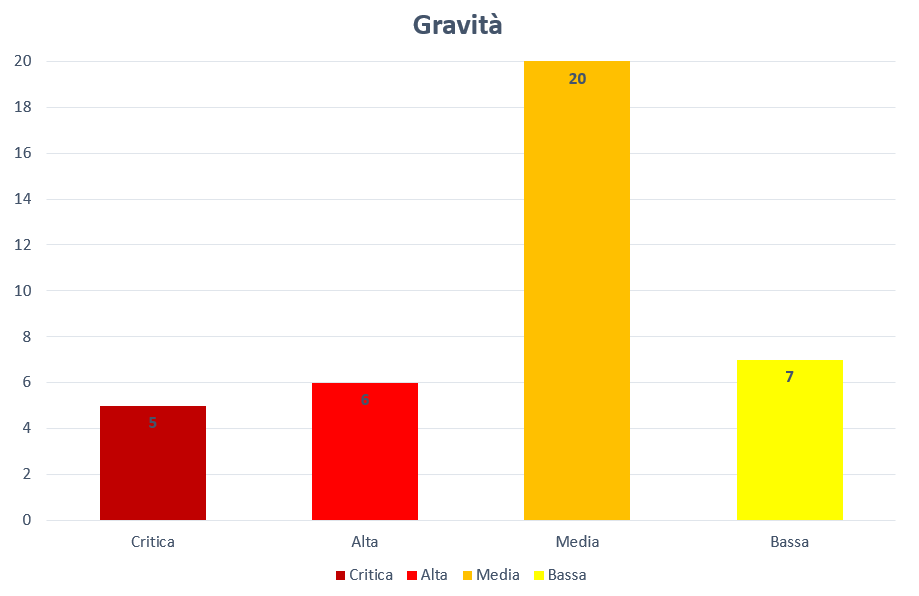
\includegraphics[width=0.9\textwidth]{capitoli/figure/bar-chart.png}
    \caption{Ortogramma riassuntivo dei rilevamenti}
\end{figure}

\begin{figure}[h]
    \centering
    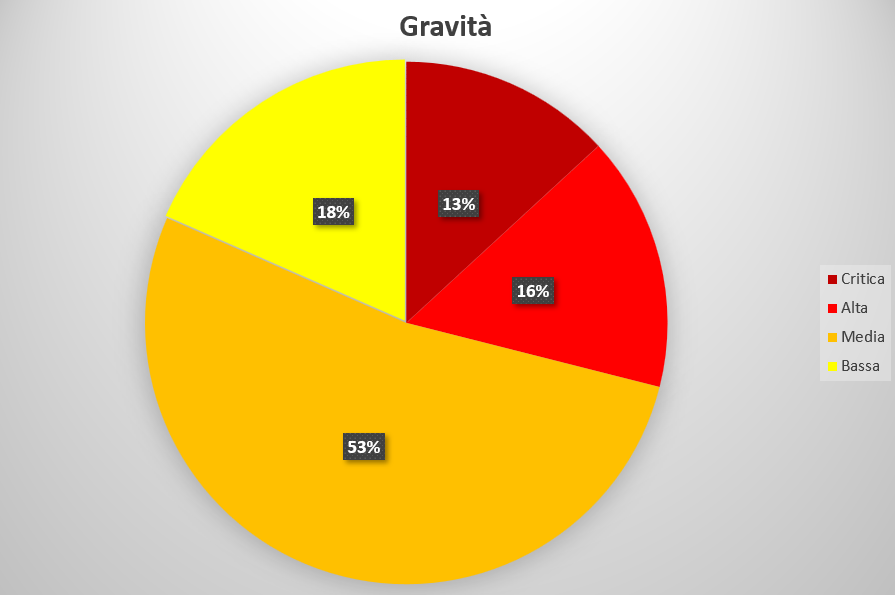
\includegraphics[width=0.9\textwidth]{capitoli/figure/pie-chart.png}
    \caption{Aerogramma riassuntivo dei rilevamenti}
\end{figure}

\section{Detailed Summary}
Di seguito saranno elencate le varie vulnerabilità riscontrate manualmente, correlate di eventuale ID e rischi associati, e saranno indicati i documenti esaustivi nei quali consultare tutte le restanti vulnerabilità riscontrate grazie a tool di rilevazione automatica.

\subsection{Information Leakage}
\begin{itemize}
    \item \textbf{Descrizione}: Informazioni sensibili non sono state protette adeguatamente o sono state inserite in risorse accessibili da utenti non autorizzati. Le informazioni trovate sono le seguenti:
        \begin{itemize}
            \item Nella discussione \textbf{Login Attacks} presente nel forum (\emph{10.0.2.4/forum}) è presente la password di \textbf{mbrown} per l'accesso alla pagina personale del forum e alla mail;
            \item Nell'account webmail di \textbf{mbrown} presente all'indirizzo \emph{10.0.2.4/webmail} è stata trovata una mail nella casella \emph{In Arrivo} che contiene le credenziali in chiaro dell'utente \textbf{root} del servizio \textbf{phpMyAdmin};
            \item Nello script che si trova al percorso \emph{/opt/backup.sh} è presente l'opzione \texttt{-pass pass:<PASSWORD>} con la password specificata in chiaro;
            \item Nella cartella \emph{.ssh} dell'utente \textbf{mbrown}, è presente un file \emph{downloadkey} che è una copia della chiave privata di tale utente, però i permessi consentono la lettura anche ad altri utenti.
        \end{itemize}
    \item \textbf{Rischi associati}: La presenza di queste informazioni permette la compromissione dell'utente \textbf{mbrown}, di tutti i database presenti in \textbf{phpMyAdmin} e dell'intero sistema, permettendo ad un attaccante di effettuare il login prima come utente \textbf{suoder} (in particolare l'utente \textbf{swillard}) e, successivamente, come utente \textbf{root}.
    \item \textbf{Soluzione}:
        \begin{itemize}
            \item Cancellare il thread \textbf{Login Attacks} dal forum;
            \item Cancellare la mail contenente la password dell'utente \textbf{root} di \textbf{phpMyAdmin} e non usare questo metodo per scambiare informazioni sensibili;
            \item Utilizzare come password un file \texttt{.key} protetto da password o, in ogni caso, con permessi tali da limitare la lettura solo agli utenti autorizzati;
            \item Rimuovere il file \emph{/home/mbrown/.ssh/downloadkey} o specificare dei permessi adeguati in modo da renderlo leggibile solo all'utente \textbf{mbrown}
        \end{itemize}
    \item \textbf{ID di riferimento}: CWE-200: Exposure of Sensitive Information to an Unauthorized Actor;
    \item \textbf{Riferimenti}: \url{https://cwe.mitre.org/data/definitions/200.html}.
\end{itemize}

\subsection{Impiego di password deboli}
\begin{itemize}
    \item \textbf{Descrizione}: Per accedere al sistema e ai servizi vengono utilizzate le stesse password o, in ogni caso, password facilmente compromissibili;
    \item \textbf{Rischi associati}: Un attaccante potrebbe entrare in possesso degli hash delle password e tramite strumenti di \emph{Offline Password Cracking} come \texttt{john} o \texttt{hashcat} potrebbe riuscire a forzare con successo le password degli utenti tramite attacco a dizionario, compromettendo il sistema;
    \item \textbf{Soluzione}: Utilizzare password diverse per ogni servizio e impiegare dei requisiti di password più stringenti, come combinazioni di caratteri alfanumerici e caratteri speciali (anche combinazioni di maiuscole e minuscole) specificando anche una lunghezza minima;
    \item \textbf{ID di riferimento}: CWE-1391: Use of Weak Credentials, CWE-521: Weak Password Requirements
    \item \textbf{Riferimenti}: \url{https://cwe.mitre.org/data/definitions/1391.html}, \url{https://cwe.mitre.org/data/definitions/521.html}.
\end{itemize}

\subsection{Rilevamenti effettuati da \emph{Nessus}}
Con il tool \emph{Nessus} sono stati generati due report, entrambi posti nella cartella \emph{Report} e con il nome \textbf{De-ICE\_scan\_nessus.pdf} e \textbf{De-ICE\_scan\_nessus\_web.pdf}.

\subsection{Rilevamenti effettuati da \emph{OpenVAS}}
Con il tool \emph{OpenVAS} è stato generato un solo report, posto nella cartella \emph{Report} e con il nome \textbf{De-ICE\_scan\_openvas.pdf}.

\subsection{Rilevamenti effettuati da \emph{OWASP ZAP}}
Con il tool \emph{OWASP ZAP} è stato generato un solo report, posto nella cartella \emph{Report} e con il nome \textbf{De-ICE-ZAP-Report.html}.

\subsection{Rilevamenti effettuati da \emph{Paros}}
Con il tool \emph{Paros} è stato generato un solo report, posto nella cartella \emph{Report} e con il nome \textbf{paros-report.htm}.

\subsection{Rilevamenti effettuati da \emph{Nikto}}
Con il tool \emph{Nikto} è stato generato un solo report, posto nella cartella \emph{Report} e con il nome \textbf{nikto-report.html}.